\subsection{A/D konverter}
\label{ADKonverter}
%
A/D konverter er en forkortelse for \textit{Analog-to-Digital Converter} og dens formål er, som navnet angiver, at oversætte et analogt signal til et digitalt signal. En analog spænding er ikke kvantificeret og kan derfor repræsenteres med alle reelle tal. Grunden til at A/D konverteren implementeres er for at aktivere de korrekte filtre, afhængigt af om der skrues op eller ned for stereovolumenkontrollen. For at de korrekte filtre aktiveres sendes outputtet fra A/D konverteren til tre multipleksere, hvor filtrene er forbundet, jævnfør \fullref{Multipleksere}. 

En primitiv A/D konverter, kan sammenligne en input spændning med en kendt referencespændning, og via en stepfunktion angive om den målte inputspænding er over eller under referencen, hvor referencespændingen i dette tilfælde er den positive forsyningsspænding $+V_F$ på 5V. A/D konverteren angiver derfor ikke nøjagtigt hvad den målte spændning er, men angiver i stedet om den målte spænding hører til i kategorien “over” eller “under” i forhold til en referencen. En primitiv A/D konverter svarer derfor til hvad en komparator gør, jævnfør \fullref{Komparator}. 

En mere sofistikeret A/D konverter kan sammenligne inputspændingen med flere forskellige kendte spændinger, som er mindre end referensenspændingen. Her udvides kvantificeringen fra at være en simpel stepfunktion, til at bestå af flere steps med hver deres grænse. Den højeste og laveste referencespænding er afgørende for hvilket område der kan måles inden for, hvor den højeste er forbundet til $+V_F$ og den laveste er forbundet til jord. For at målingen bliver nøjagtige, er det nødvendigt at inputspændingen befinder sig inden for referencespændet, mellem $+V_F$ og jord. Måles inputspænding til at være højere end den højeste referencespænding, $+V_F$, angiver A/D konverteren, i bedste fald, at målingen var højere end $+V_F$. Nøjagtigheden forringes da det målte ikke længere er sammenlignligt med noget højere, hvorfor spændet teoretisk set kvantificeres fra at gå fra den højeste referencespænding, $+V_F$, til en ukendt spænding derover.

A/D konverteres vigtigste opgave er derfor at måle og kvantificere en analog spænding i forhold til en referencespænding, for dernæst at konvertere den målte analoge spænding til en digital, binær, talkode. At et digitalt signal er binært referer til at det følger 2-talsystemet og derfor kun kan være 1 (højt) eller 0 (lavt). Hvert output kan derfor gengives som et af de to stadier, hvilket medfører at opløsningen hvormed en A/D konverter kan konvertere og videregive et analogt signal til et digitalt signal, i høj grad afhænger af antallet af digitale outputs. 
Matematisk kan det udledes ved at opløfte antallet af outputs N i grundtallet 2, $2^N$, hvor N er antallet af outputs og 2 er antal stadier outputtet kan gengive. Et enkelt digitalt output kan udtrykke forskellen mellem to spændinger og kan matematisk udledes som:
%
\begin{equation}
	2^1 = 2
\end{equation}
%
To digitale outputs kan udtrykke forskellen mellem fire spændinger og udledes som:
%
\begin{equation}
	2^2 = 4
\end{equation}  
%
Således bestemmer antallet af binære outputs fra A/D konverteren opløsningen, der kan konverteres med. Hver gang der tilføreres et ekstra binært output, fordobles opløsningen og kvantificeringen af inputspændingen kan derfor foregå dobbelt så nøjagtigt.
Opløsningen af A/D konverteren brugt i kredsløbet, udledes ved:
%
\begin{equation}
	2^8 = 256
\end{equation}
% 
Nøjagtigheden kan tilnærmes ved at subtrahere den laveste referencespænding, $V_{in-}$ der er koblet til jord, fra den største, $+V_F$, og derefter dividere med antallet af kvantificerede spænd, hvor en bit giver to spænd. Matematisk kan det udledes ved:
%
\begin{equation}
\frac{+V_{F}-V_{in-}}{2^N}
\label{equ:Noejagtighed}
\end{equation}
%
Fra \autoref{equ:Noejagtighed} udledes det interval inputspændingen kan være indenfor, som er dækket af den fulde referencespænding $+V_F$. Herefter divideres den fulde referencespænding med antallet af outputs fra A/D konverteren, opløftet i antallet af stadier én bit kan befinde sig i. Nøjagtigheden af A/D konverteren udregnes derfor til:
%
\begin{equation}
	\frac{+5V-0V}{2^8} = \frac{+5V}{256} = 0.0195V = 19.5mV
\end{equation}
%
Nøjagtigheden kan også udtrykkes som et resultat af referencespændingen divideret med opløsningen:
%
\begin{equation}
	\textit{Nøjagtighed} = \frac{\textit{referencespænding}}{\textit{opløsning}}
\end{equation}
%
Hver gang der måles konverterer A/D konverteren outputtet fra dobbeltensretteren til en digital binær talkode. Målingerne bliver foretaget med en klokfrekvens på $\approx$1000Hz, svarende til at hver bit bliver målt ved $\approx$125Hz.

Talkodens længde, og dermed A/D konvertererens opløsning, afgøres af antallet outputs, da hvert output bidrager med et tal i koden. For at sikre en detaljeret måling af det analoge inputsignal, er det nødvendigt at foretage målingerne minimum dobbelt så ofte, som frekvensen af det målte signal fra dobbeltensretter. Der skal altså flere målinger til inden for den samme periode for at sikre målingernes validitet. Et stort antal målinger inden for den samme periode vil styrke validiteten af målingen, men vil ikke gøre målingen mere nøjagtig. Det er derfor et spørgsmål om resurseforbrug og validitet, der afgør hvilken frekvens der skal styrer hvornår målingerne foretages.
%
\begin{figure}[H]
	\centering
	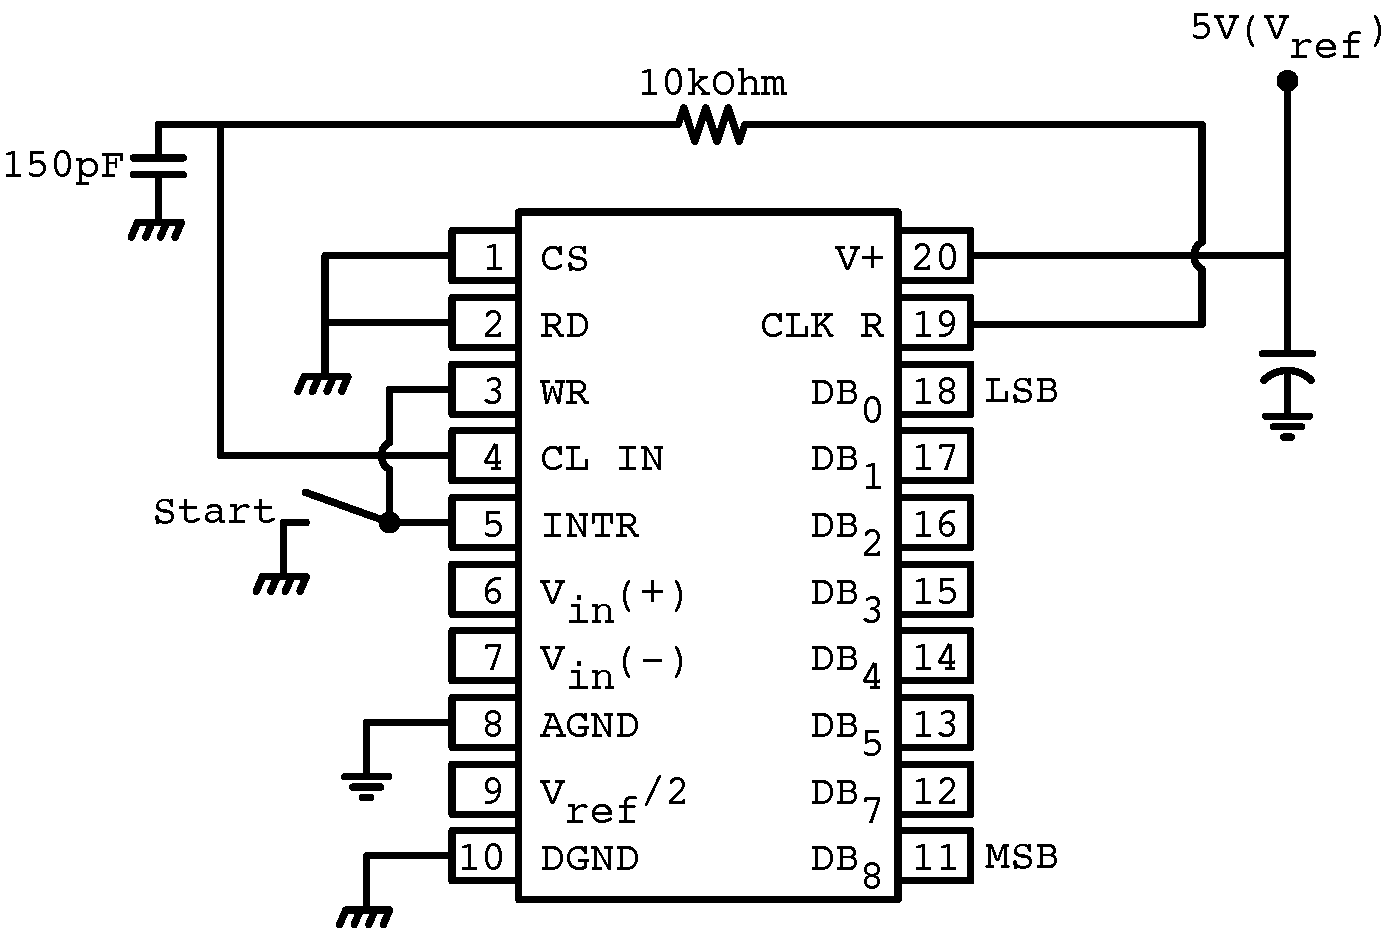
\includegraphics[resolution=300,scale=\circuitSize]{Figure/Circuits/ADC_FreeRunning}
	\caption{Kredsløbsdiagram for en \textit{Free Running} opkobling af A/D konverteren.\parencite[s. 11]{PDF:ADC}}
	\label{fig:ADC_FreeRunning}
\end{figure}
\noindent
%
At A/D konverteren forbindes som \textit{Free Running}, angiver at A/D konverteren foretager målingerne uafbrudt med en bestemt klokfrekvens, hvilket fremgår af ben 19 på \autoref{fig:ADC_FreeRunning}. Ved en standard opkobling i \textit{Free Running} anvendes en kondensator på 150pF, som er forbundet efter en modstand på $10k\Omega$, denne opkobling vil have en klokfrekvens på 600kHz. klokfrekvensen beregnes ved følgende udtryk:
%
\begin{equation}
	f_{CLK} = \frac{1}{1.1*R*C}
	\label{equ:KlokFrekvens}
\end{equation}
%
Hvor $f_{CLK}$ angiver klokfrekvensen, $R$ er modstanden på $10k\Omega$ og C er kondensatoren. Som tidligere nævnt vil målingerne blive foretaget med en klokfrekvens på $\approx$1000Hz, så baseret på \autoref{equ:KlokFrekvens} er det muligt at beregne hvilken værdi kondensatoren skal have:
%
\begin{equation}
	C = \frac{1}{1.1*R*f_{CLK}} = \frac{1}{1.1*10k\Omega*1000Hz} = 0.1\mu F
\end{equation}
%
Med en kondensator på $0.1\mu F$ vil klokfrekvensen reelt blive mindre end 1000Hz:
%
\begin{equation}
	f_{CLK} = \frac{1}{1.1*10k\Omega*0.1\mu F} = 909.09Hz
\end{equation}
%
For at A/D konverteren begynder at foretage målinger skal $\overline{INTR}$, som er forbundet til $\overline{WR}$, registrere en puls. Som illustreret på \autoref{fig:ADC_FreeRunning} styres pulsen af en kontakt, der i dette tilfælde implementeres, som en del af brugergrænsefladen, jævnfør \fullref{Brugergraenseflade}. \\[5mm]
%
Selvom at A/D konverteren har otte bits som output, og en opløsning på 256, bliver der i styresystemet kun gjort brug af de fire mest betydende bits. Med fire bits fås en opløsning på 16. Fordelen ved at bruge de fire mest betydende bits er at det kræver en større spændingsforskel før de individuelle bits skifter stadie. Hver af de fire bits er koblet til indgangen på en multiplekser, som sørger for, afhængigt af hvilket stadie den pågældende bit er i, at filtrene enten aktiveres eller deaktiveres. 

For at beregne hvor stor en spænding der skal til for at hver bit skifter stadie én gang, anvendes følgende udtryk:
%
\begin{equation}
	V = 2^n*\frac{+V_F}{2^N}
\end{equation}
% 
Hvor n angiver hvilken bit spændingen beregnes ud fra, N angiver opløsningen som i det specifikke tilfælde er $2^4 = 16$. Så for den første bit $DB_4$, illustreret på \autoref{fig:ADC_FreeRunning}, er det muligt at beregne den spænding der skal til for at den skifter stadie:
%
\begin{equation}
	2^0*\frac{5V}{16} = 0.3125V
\end{equation}
% 
For den næste bit $DB_5$:
%
\begin{equation}
	2^1*\frac{5V}{16} = 0.625V
\end{equation}
%
For den tredje bit $DB_6$:
%
\begin{equation}
	2^2*\frac{5V}{16} = 1.25V
\end{equation}
%
For den fjerde, og mest betydende bit, $DB_7$:
%
\begin{equation}
	2^3*\frac{5V}{16} = 2.5V
\end{equation}
%
De forgående beregninger relaterer sig kun til skiftet fra et stadie til et andet, og ikke tilbage igen, så for at én bit opnår begge stadier (0 og 1) så skal spændingen fordobles. For den mest betydende bit $DB_7$ betyder det at spændingen principielt skal være 5V for at kunne skifte mellem de to stadier. 
%
\begin{figure}[H]
	\centering
	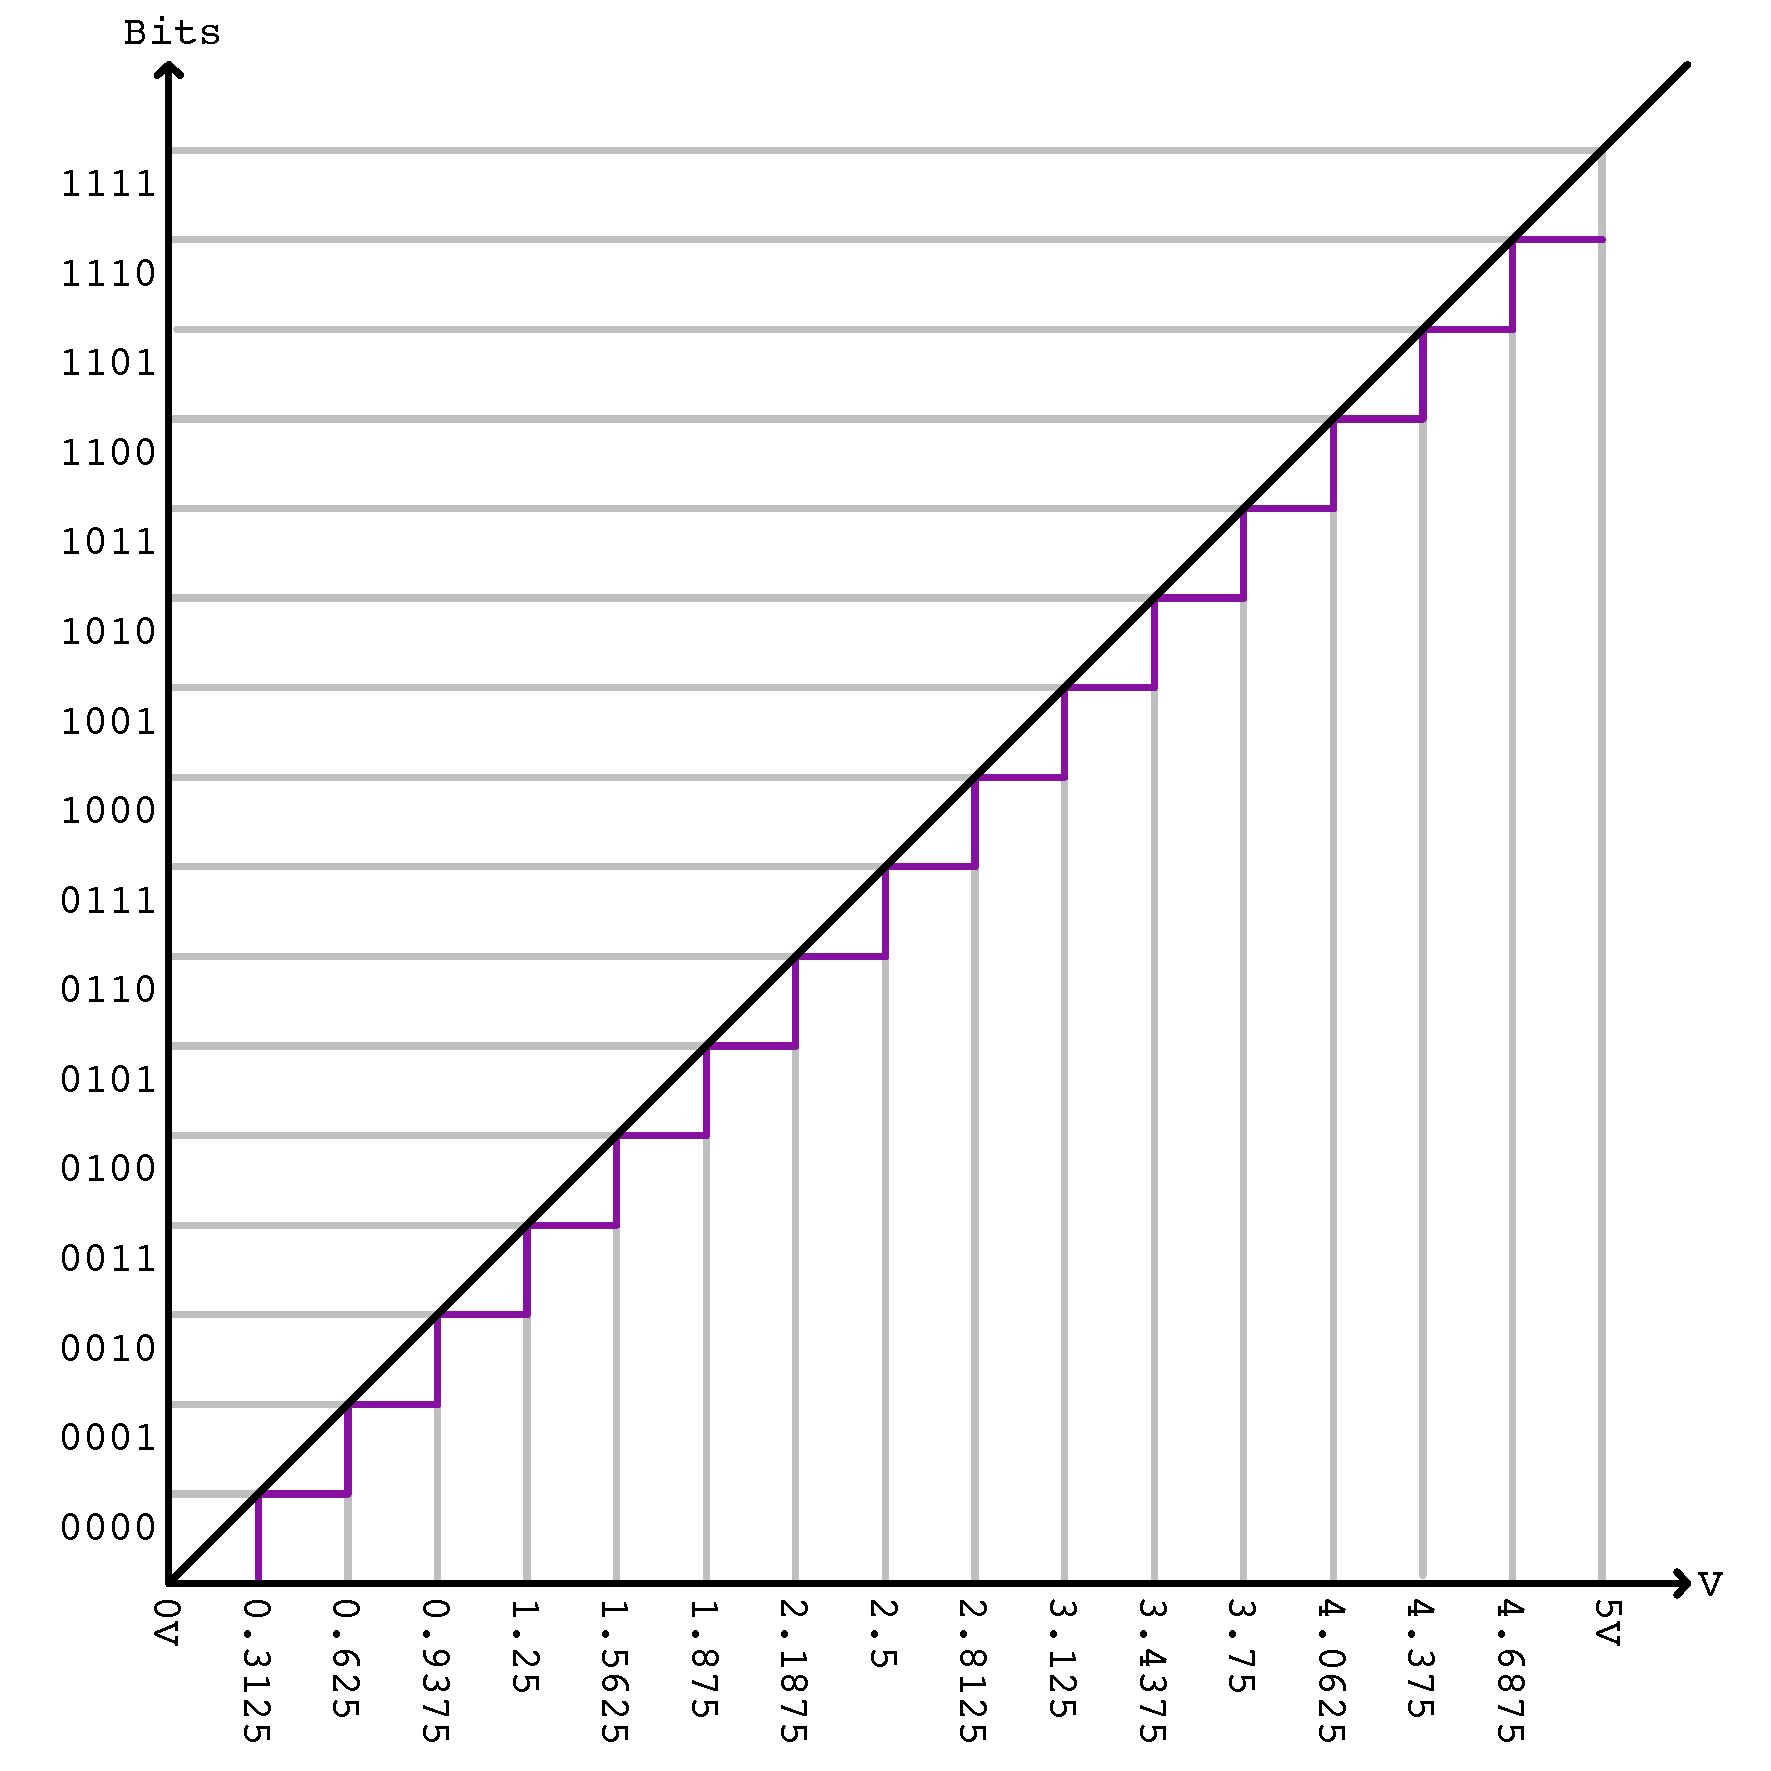
\includegraphics[resolution=300,scale=\circuitSize]{Figure/Circuits/Bits.pdf}
	\caption{Sammenhæng mellem spændning [V] og aktivering af de fire bits.}
	\label{fig:ADC_Bits}
\end{figure}
\noindent
%
På \autoref{fig:ADC_Bits} illustreres det i kronologisk rækkefølge ved hvilken spænding hver af de 16 bits skifter stadie, og dermed hvilket output A/D konverteren sender til multiplekserne. Det vil i  \fullref{SystemSammenSaetningOgAccepttest} blive undersøgt om disse spændinger også er en realitet i praksis og dertil om aktiveringen af de fire bits foregår i overensstemmelse med hvilke filtre der skal benyttes. A/D konverteren der implementeres i styresystemet er af typen \textit{ADC0803LCN}, \parencite{PDF:ADC}.
